% =====================================================================
%  High-level U-GNN architecture  (reference: sophisticated-oarfish-9)
%  ---------------------------------------------------------------------
%  Staircase-U layout, symbolic (macro-driven) size labels, main signal
%  path + skip connections + STUBBED conditioning / time side-inputs.
%
%  Reference run: WRA medium-large "Ablation 1: Baseline" (T = 1, pure
%  spatial U-GNN).  3 encoder levels, gamma = [1, 2, 2]:
%     N -> N (Enc0, no pool) -> N/2 (Enc1) -> N/4 (Enc2) -> bottleneck
%  uniform C channels at every level; input_proj 1->C, output_proj C->1.
%
%  Compile:  pdflatex highlevel_ugnn_beamer.tex   (or lualatex)
%  To drop into an existing deck: copy the tikzpicture (inside \resizebox)
%  into your own frame.
% =====================================================================
\documentclass[aspectratio=169]{beamer}   % <- 43 for 4:3 slides
\usepackage{amsmath}
\usepackage{bm}
\usepackage{tikz}
\usetikzlibrary{positioning, arrows.meta, calc, fit, backgrounds}

% ---------------------------------------------------------------------
%  EDITABLE PARAMETERS
% ---------------------------------------------------------------------
% --- Geometry of the staircase-U (change these to reshape the whole U) -
\newcommand{\halfspan}{4.0}   % half horizontal span at the top level (cm)
\newcommand{\stepx}{1.05}     % horizontal inward step per depth level
\newcommand{\stepy}{1.20}     % vertical step down per depth level
% Encoder node at depth d:  (-\halfspan + d*\stepx , -d*\stepy)
% Decoder node at depth d:  ( \halfspan - d*\stepx , -d*\stepy)
% Bottleneck:               ( 0 , -3*\stepy )

% --- Symbolic size labels (redefine to concrete numbers if desired,
%     e.g. \renewcommand{\Nfull}{400}, \Nhalf{200}, \Nquart{100}, \Cch{64}) -
\newcommand{\Nfull}{N}
\newcommand{\Nhalf}{N/2}
\newcommand{\Nquart}{N/4}
\newcommand{\Cch}{C}

% ---------------------------------------------------------------------
%  STYLES  (appearance is centralised here)
% ---------------------------------------------------------------------
\tikzset{
  % --- nodes ---
  block/.style      = {rounded corners=2pt, draw=blue!55!black, fill=blue!8,
                       line width=0.6pt, align=center, inner sep=4pt,
                       minimum width=1.5cm, minimum height=0.95cm},
  bottleneck/.style = {rounded corners=2pt, draw=orange!80!black, fill=orange!15,
                       line width=0.7pt, align=center, inner sep=4pt,
                       minimum width=1.7cm, minimum height=0.95cm},
  proj/.style       = {rounded corners=1pt, draw=black!55, fill=black!6,
                       align=center, font=\scriptsize, inner sep=3pt,
                       minimum height=0.8cm},
  sideinput/.style  = {rounded corners=2pt, draw=violet!60!black, fill=violet!8,
                       dashed, align=center, font=\scriptsize, inner sep=3pt,
                       minimum width=1.7cm, minimum height=0.8cm},
  io/.style         = {font=\normalsize},
  % --- edges ---
  sig/.style        = {-{Stealth[length=2.4mm]}, line width=1.0pt, black},
  skip/.style       = {-{Stealth[length=2.0mm]}, line width=0.8pt,
                       blue!60, dashed},
  cond/.style       = {-{Stealth[length=1.8mm]}, line width=0.7pt,
                       violet!55, densely dotted},
  gam/.style        = {font=\tiny\itshape, text=black!55},
  note/.style       = {font=\scriptsize, text=violet!60!black, align=center},
}

\begin{document}

\begin{frame}{U-GNN denoiser --- high-level architecture}
\centering
% \resizebox keeps the figure within the slide regardless of the cm units
% chosen above.  Delete it if you prefer to control the scale by hand.
\resizebox{\linewidth}{!}{%
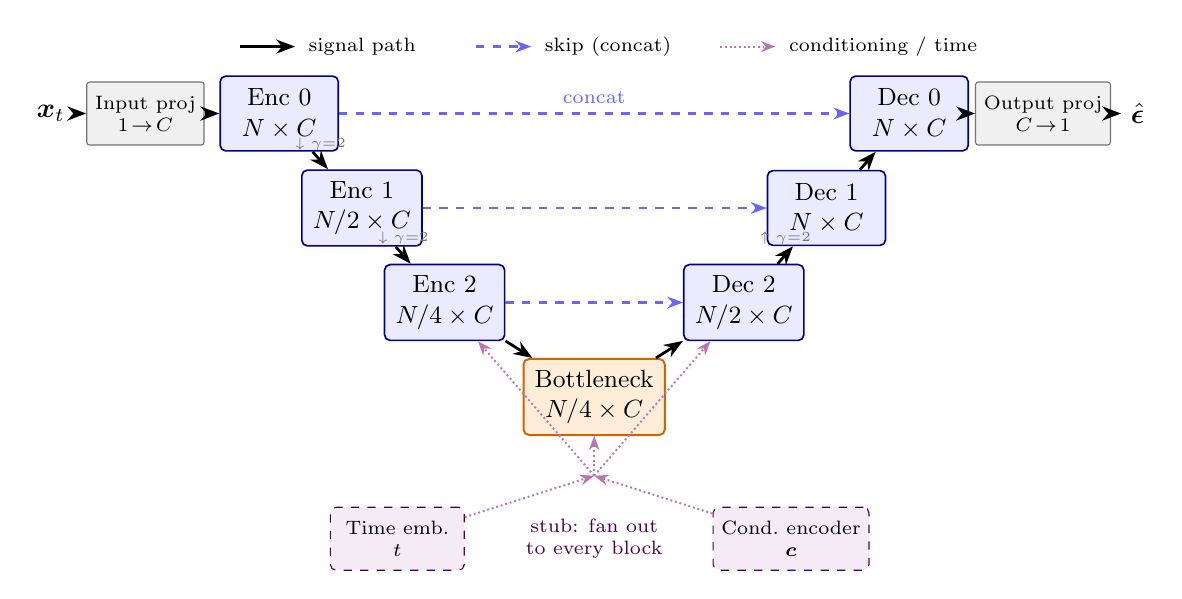
\begin{tikzpicture}[font=\small]

  % ===================================================================
  %  MAIN BLOCKS
  % ===================================================================
  % --- input / output projections + I/O tensors ---
  \node[io]   (xt)  at (-\halfspan-2.9, 0) {$\bm{x}_t$};
  \node[proj] (in)  at (-\halfspan-1.7, 0) {Input proj\\$1\!\to\!\Cch$};
  \node[proj] (out) at ( \halfspan+1.7, 0) {Output proj\\$\Cch\!\to\!1$};
  \node[io]   (eps) at ( \halfspan+2.9, 0) {$\hat{\bm{\epsilon}}$};

  % --- encoder column (steps down-right) ---
  \node[block] (e0) at (-\halfspan + 0*\stepx, -0*\stepy) {Enc 0\\$\Nfull\times\Cch$};
  \node[block] (e1) at (-\halfspan + 1*\stepx, -1*\stepy) {Enc 1\\$\Nhalf\times\Cch$};
  \node[block] (e2) at (-\halfspan + 2*\stepx, -2*\stepy) {Enc 2\\$\Nquart\times\Cch$};

  % --- bottleneck (base of the U) ---
  \node[bottleneck] (bn) at (0, -3*\stepy) {Bottleneck\\$\Nquart\times\Cch$};

  % --- decoder column (steps up-right) ---
  \node[block] (d2) at (\halfspan - 2*\stepx, -2*\stepy) {Dec 2\\$\Nhalf\times\Cch$};
  \node[block] (d1) at (\halfspan - 1*\stepx, -1*\stepy) {Dec 1\\$\Nfull\times\Cch$};
  \node[block] (d0) at (\halfspan - 0*\stepx, -0*\stepy) {Dec 0\\$\Nfull\times\Cch$};

  % ===================================================================
  %  MAIN SIGNAL PATH (spine)
  % ===================================================================
  \draw[sig] (xt) -- (in);
  \draw[sig] (in) -- (e0);
  \draw[sig] (e0) -- (e1) node[gam, midway, above] {$\downarrow\gamma{=}2$};
  \draw[sig] (e1) -- (e2) node[gam, midway, above] {$\downarrow\gamma{=}2$};
  \draw[sig] (e2) -- (bn);
  \draw[sig] (bn) -- (d2);
  \draw[sig] (d2) -- (d1) node[gam, midway, above] {$\uparrow\gamma{=}2$};
  \draw[sig] (d1) -- (d0);
  \draw[sig] (d0) -- (out);
  \draw[sig] (out) -- (eps);
  % Note: the up-sample on bn->d2 is implied by the Dec2 size label; add a
  % "$\uparrow\gamma{=}2$" node above it here if you want it spelled out.

  % ===================================================================
  %  SKIP CONNECTIONS  (encoder -> decoder, matched depth, concat)
  % ===================================================================
  \draw[skip] (e0) -- (d0) node[midway, above, font=\scriptsize, text=blue!60] {concat};
  \draw[skip] (e1) -- (d1);
  \draw[skip] (e2) -- (d2);

  % ===================================================================
  %  SIDE-INPUT STUBS  (conditioning + time)   --- wire to blocks later
  % -------------------------------------------------------------------
  %  Currently fanned only to the deepest three blocks for clarity.
  %  To feed every block, add more  \draw[cond] (cbus) -- (<block>);  lines
  %  (or a \blocktap macro) targeting e0, e1, d0, d1 as well.
  % ===================================================================
  \coordinate (cbus) at (0, {-3*\stepy - 1.0});                  % fan-out junction
  \node[sideinput] (temb) at (-2.5, {-3*\stepy - 1.8}) {Time emb.\\$t$};
  \node[sideinput] (cenc) at ( 2.5, {-3*\stepy - 1.8}) {Cond.\ encoder\\$\bm{c}$};

  \draw[cond] (temb) -- (cbus);
  \draw[cond] (cenc) -- (cbus);
  \draw[cond] (cbus) -- (e2);
  \draw[cond] (cbus) -- (bn);
  \draw[cond] (cbus) -- (d2);
  \node[note] at (0, {-3*\stepy - 1.8}) {stub: fan out\\to every block};

  % ===================================================================
  %  LEGEND  (delete this scope if not wanted)
  % ===================================================================
  \begin{scope}[shift={(-\halfspan-0.5, 0.85)}]
    \draw[sig]  (0,0)   -- (0.7,0);  \node[anchor=west, font=\scriptsize] at (0.75,0) {signal path};
    \draw[skip] (3.0,0) -- (3.7,0);  \node[anchor=west, font=\scriptsize] at (3.75,0) {skip (concat)};
    \draw[cond] (6.1,0) -- (6.8,0);  \node[anchor=west, font=\scriptsize] at (6.85,0) {conditioning / time};
  \end{scope}

\end{tikzpicture}
}%
\end{frame}

\end{document}
